\documentclass[11pt]{article}

\usepackage{subcaption}
\usepackage{latexsym}
\usepackage{amsmath}
\usepackage{amssymb}
\usepackage{amsthm}
\usepackage{graphicx}
\usepackage{wrapfig}
\usepackage{pseudocode}
\usepackage{url}
\usepackage[backref, colorlinks=true, citecolor=red, urlcolor=blue, pdfauthor={Student}]{hyperref}


\newcommand{\handout}[5]{
  \noindent
  \begin{center}
  \framebox{
    \vbox{
      \hbox to 5.78in { {\bf Advanced Algorithms} \hfill #2 }
      \vspace{4mm}
      \hbox to 5.78in { {\Large \hfill #5  \hfill} }
      \vspace{2mm}
      \hbox to 5.78in { {\em #3 \hfill #4} }
    }
  }
  \end{center}
  \vspace*{4mm}
}

\newcommand{\lecture}[4]{\handout{#1}{#2}{#3}{}{Report for #1}}

\newtheorem{theorem}{Theorem}
\newtheorem{corollary}[theorem]{Corollary}
\newtheorem{lemma}[theorem]{Lemma}
\newtheorem{observation}[theorem]{Observation}
\newtheorem{proposition}[theorem]{Proposition}
\newtheorem{definition}[theorem]{Definition}
\newtheorem{claim}[theorem]{Claim}
\newtheorem{fact}[theorem]{Fact}
\newtheorem{assumption}[theorem]{Assumption}

\topmargin 0pt
\advance \topmargin by -\headheight
\advance \topmargin by -\headsep
\textheight 8.9in
\oddsidemargin 0pt
\evensidemargin \oddsidemargin
\marginparwidth 0.5in
\textwidth 6.5in

\parindent 0in
\parskip 1.5ex

\begin{document}

\lecture{Advance Algorithm Programming Assignment 1 }{Fall 2017}{Your name}{Srivats Bharadwaj}

\textit{In geometry, a triangulation is a subdivision of a planar object into triangles, and by extension the subdivision of a higher-dimension geometric object into simplices. Triangulations of a three-dimensional volume would involve subdividing it into tetrahedra ("pyramids" of various shapes and sizes) packed together.} \textbf{-wiki}

In this assignment it is proposed to study different triangulation techniques to get acquainted with the problem of triangulation. Such techniques are proposed to be explored: building of convex hull, Delaunay triangulation (and corresponding Voronoi diagram), provide an “alpha” filtering (aka. alpha shaping)  and finally apply the “crust” algorithm.

Given ideas proposed to be implemented using c-language and the package qhull that may be found here: \href{http://www.qhull.org}{qhull}.
The “qhull” package used as a core for final program that is call it mainly to build convex hull and Delaunay triangulation.

For visualization purposes, it was proposed to use “freeglut”.

Also, as to begin with the skeleton code was given that may be found on appropriate \href{https://github.com/jmlien/cshape}{git}.

For testing purposes the next data has been used (fig.~\ref{fig:points})

\begin{figure}[h]
    \begin{subfigure}{.3\textwidth}
        \centering
        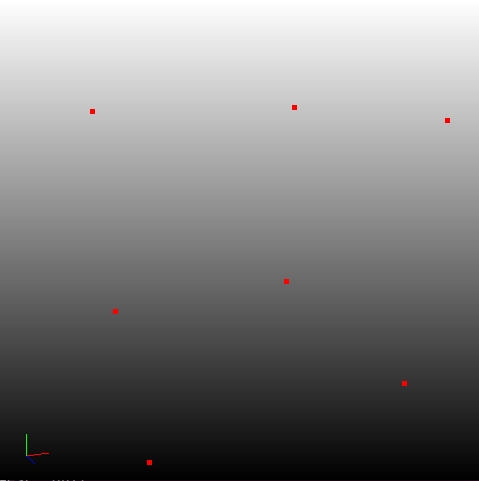
\includegraphics[width=.8\textwidth]{FIGS/points/points_cube}
        \caption{Cube: data points}
    \end{subfigure}
    \begin{subfigure}{.3\textwidth}
        \centering
        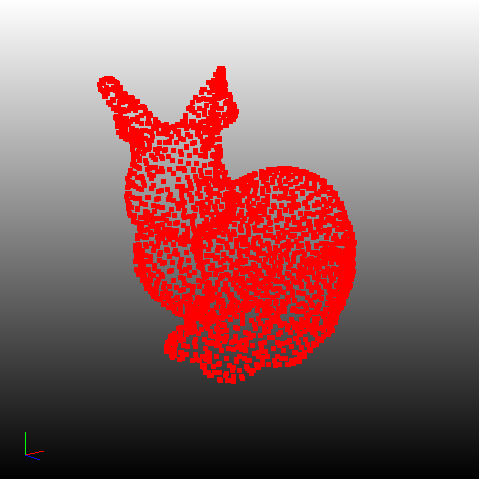
\includegraphics[width=.8\textwidth]{FIGS/points/points_bunny}
        \caption{Bunny: data points}
    \end{subfigure}
    \begin{subfigure}{.3\textwidth}
        \centering
        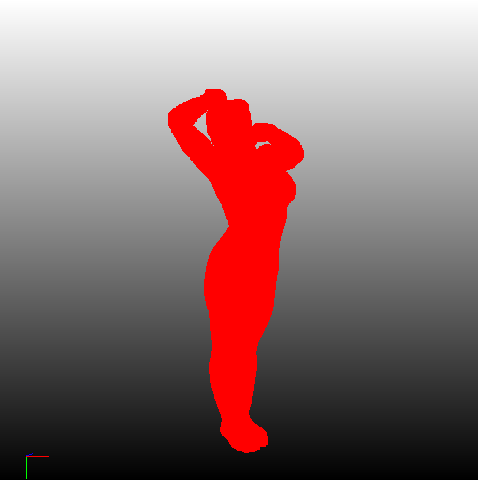
\includegraphics[width=.8\textwidth]{FIGS/points/points_woman}
        \caption{Woman: data points}
    \end{subfigure}
    \caption{Testing samples}
    \label{fig:points}
\end{figure}


\section{Convex Hull}
\textit{In mathematics, the convex hull or convex envelope of a set X of points in the Euclidean plane or in a Euclidean space (or, more generally, in an affine space over the reals) is the smallest convex set that contains X. For instance, when X is a bounded subset of the plane, the convex hull may be visualized as the shape enclosed by a rubber band stretched around X.} \textbf{-wiki}

To build the convex hull using “qhull” package noting special should be done – just pass the points in format of array of coordinates into the “qhull” and get the result back. To build simple convex hull the next “qhull” options string was used: \textbf{qhull QJ Pp}. The “qhull” output is a set of triangles: 3-points groups set, and so it is possible to build a 3d figure upon this data.

Examples of convex hull built in this way are shown below on fig.~\ref{fig:convex}
\begin{figure}[h]
    \begin{subfigure}{.3\textwidth}
        \centering
        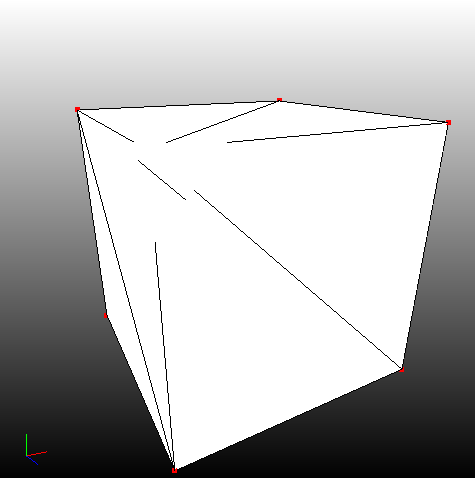
\includegraphics[width=.8\textwidth]{FIGS/convex_hull/convex_cube}
        \caption{Cube: convex hull}
    \end{subfigure}
    \begin{subfigure}{.3\textwidth}
        \centering
        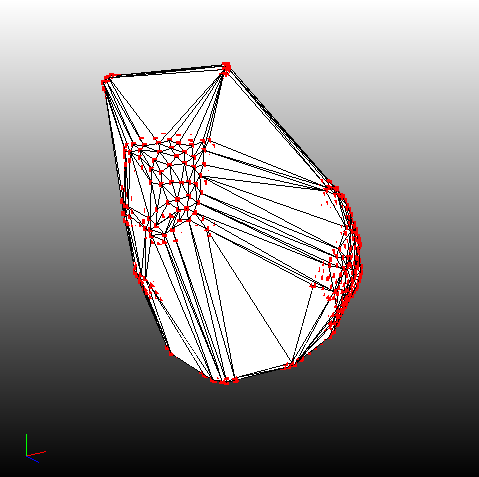
\includegraphics[width=.8\textwidth]{FIGS/convex_hull/convex_bunny}
        \caption{Bunny: convex hull}
    \end{subfigure}
    \begin{subfigure}{.3\textwidth}
        \centering
        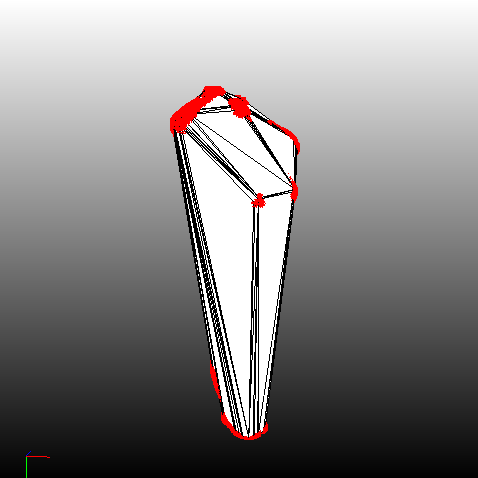
\includegraphics[width=.8\textwidth]{FIGS/convex_hull/convex_woman}
        \caption{Woman: convex hull}
    \end{subfigure}
    \caption{Convex hull}
    \label{fig:convex}
\end{figure}

Just as expected, the convex hull is not good enough for complex objects – most of all object's details remain hidden.

\section{Delaunay triangulation}
\textit{In mathematics and computational geometry, a Delaunay triangulation for a given set P of discrete points in a plane is a triangulation DT(P) such that no point in P is inside the circumcircle of any triangle in DT(P). Delaunay triangulations maximize the minimum angle of all the angles of the triangles in the triangulation; they tend to avoid sliver triangles. The triangulation is named after Boris Delaunay for his work on this topic from 1934.}

\textit{For a set of points on the same line there is no Delaunay triangulation (the notion of triangulation is degenerate for this case). For four or more points on the same circle (e.g., the vertices of a rectangle) the Delaunay triangulation is not unique: each of the two possible triangulations that split the quadrangle into two triangles satisfies the "Delaunay condition", i.e., the requirement that the circumcircles of all triangles have empty interiors.
By considering circumscribed spheres, the notion of Delaunay triangulation extends to three and higher dimensions. Generalizations are possible to metrics other than Euclidean distance. However, in these cases a Delaunay triangulation is not guaranteed to exist or be unique.} \textbf{-wiki}

\textit{The problem of finding the Delaunay triangulation of a set of points in d-dimensional Euclidean space can be converted to the problem of finding the convex hull of a set of points in (d+1)-dimensional space, by giving each point p an extra coordinate equal to |p|2, taking the bottom side of the convex hull, and mapping back to d-dimensional space by deleting the last coordinate.} \textbf{-wiki}

Just as mentioned in quote, to perform the Delaunay triangulation in context of the given assignment it is enough to build the convex hull for same points but lifted-up into higher dimension – add 4-th coordinate that is equal to square of the radius vector absolute value $(x^2+y^2+z^2)$ and then map the result back to 3d dimension. All this operations are already coded inside the “qhull” package and the user just should input lifted to 4th dimension points (just add the 4th coordinate mentioned above).

After the evaluation of Delaunay triangulation, qhull package will output set of tetrahedrons (instead of triangles as it was in simple convex hull): grouped by 4 points set.

Results of Delaunay triangulation that was done using \textbf{delaunay QJ Pp} options string are shown below on fig.~\ref{fig:delaunay}
\begin{figure}[h]
    \begin{subfigure}{.3\textwidth}
        \centering
        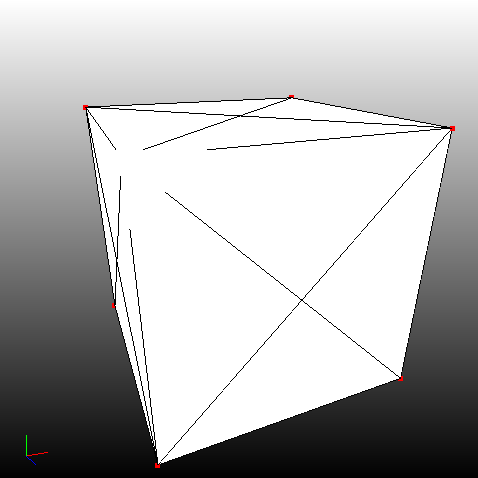
\includegraphics[width=.8\textwidth]{FIGS/delaunay/delaunay_cube}
        \caption{Cube: Delaunay}
    \end{subfigure}
    \begin{subfigure}{.3\textwidth}
        \centering
        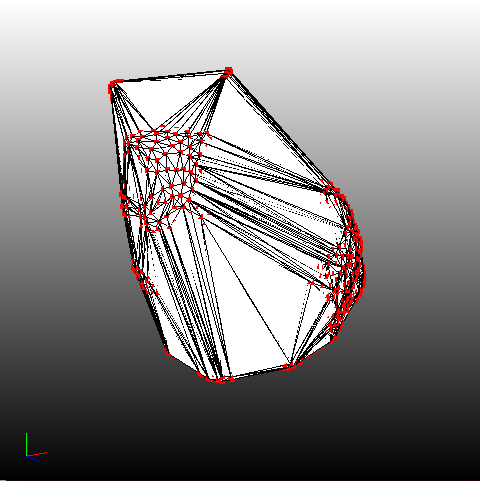
\includegraphics[width=.8\textwidth]{FIGS/delaunay/delaunay_bunny}
        \caption{Bunny: Delaunay}
    \end{subfigure}
    \begin{subfigure}{.3\textwidth}
        \centering
        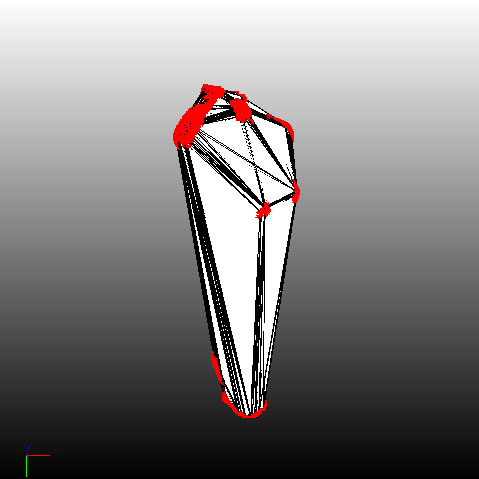
\includegraphics[width=.8\textwidth]{FIGS/delaunay/delaunay_woman}
        \caption{Woman: Delaunay}
    \end{subfigure}
    \caption{Delaunay}
    \label{fig:delaunay}
\end{figure}

The results seems same as in case of simple “convex hull” but thats not true. The given pictures shows not all the data – Delaunay triangulation contains much more triangles than “convex hull” and to achieve better results they just should be filtered.

\section{3D alpha-shape}
As it was mentioned before, the result of Delaunay triangulation requires some filtration to give better result and one of such filtration technique is named as “alpha shape”.
For a given value of $\alpha$, 
the $\alpha$-shape includes all the tetrahedra in the Delaunay triangulation which have an empty circumsphere with {\em squared radius} equal or smaller than $\alpha$.
Algorithm~\ref{alg:alphashape} sketches this idea.

{\small
	\begin{pseudocode}[shadowbox]{$\alpha$ shape}{P[1 \cdots n], \alpha}
	\label{alg:alphashape}
	\COMMENT{$P$ is a set $n$ points}\\
	D = \text{Delaunay triangulation of $P$} \\
	\FOREACH { \text{tetrahedron } t \in D} \DO
	\BEGIN
	\IF \text{the circumsphere of $t$ has squared radius larger than $\alpha$}  \DO
		\text{Remove } t
	\END
	\end{pseudocode}
}

Given ideas has been implemented using same approaches as for Delaunay triangulation. This time qhull output that is a set of tetrahedrons has been filtered: for each tetrahedron circumsphere has been evaluated (using mathematics given \href{http://www.ambrsoft.com/TrigoCalc/Sphere/Spher3D_.htm}{here}). Those tetrahedron that has zero volume (all 4 points lies on in one plane) or has larger then specified alpha square radius has been skipped.

The results are shown below on fig.~\ref{fig:alpha_bunny}, fig.~\ref{fig:alpha_woman} 
\begin{figure}[h]
    \begin{subfigure}{.22\textwidth}
        \centering
        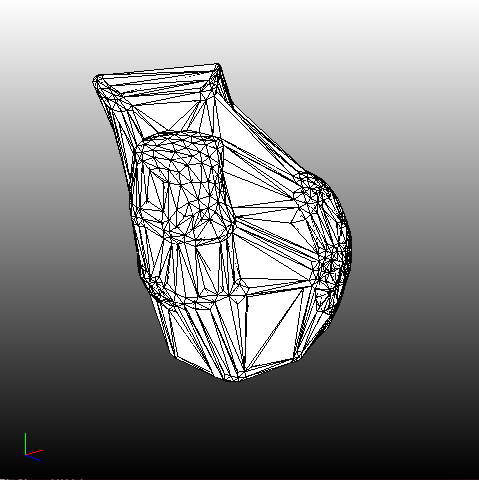
\includegraphics[width=.8\textwidth]{FIGS/alpha/alpha_bunny_100k}
        \caption{100 000}
    \end{subfigure}
    \begin{subfigure}{.22\textwidth}
        \centering
        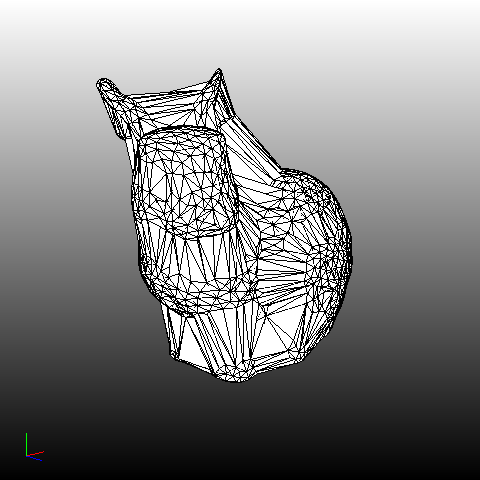
\includegraphics[width=.8\textwidth]{FIGS/alpha/alpha_bunny_20k}
        \caption{20 000}
    \end{subfigure}
    \begin{subfigure}{.22\textwidth}
        \centering
        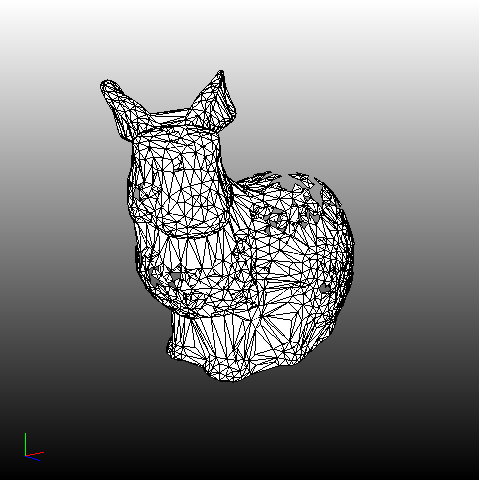
\includegraphics[width=.8\textwidth]{FIGS/alpha/alpha_bunny_5k}
        \caption{5 000}
    \end{subfigure}
    \begin{subfigure}{.22\textwidth}
        \centering
        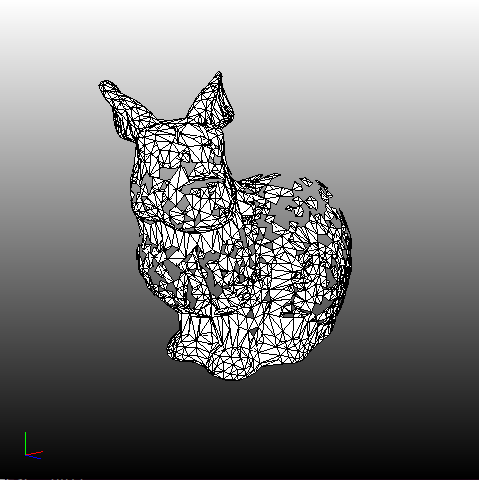
\includegraphics[width=.8\textwidth]{FIGS/alpha/alpha_bunny_2k}
        \caption{2 000}
    \end{subfigure}
    \caption{Alpha shape: bunny}
    \label{fig:alpha_bunny}
\end{figure}


\begin{figure}[h]
    \begin{subfigure}{.22\textwidth}
        \centering
        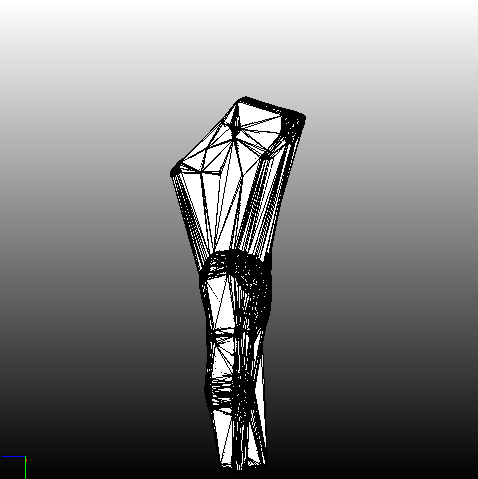
\includegraphics[width=.8\textwidth]{FIGS/alpha/alpha_woman_100k}
        \caption{100 000}
    \end{subfigure}
    \begin{subfigure}{.22\textwidth}
        \centering
        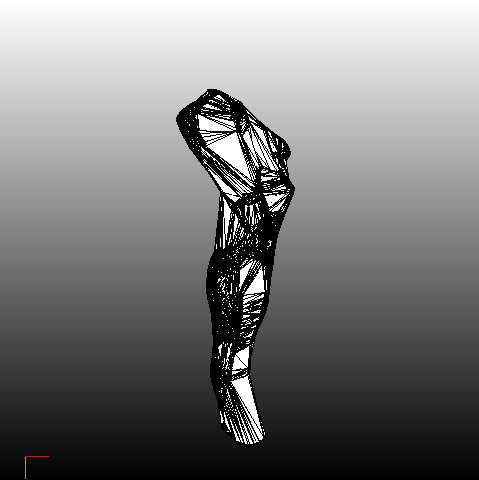
\includegraphics[width=.8\textwidth]{FIGS/alpha/alpha_woman_20k}
        \caption{20 000}
    \end{subfigure}
    \begin{subfigure}{.22\textwidth}
        \centering
        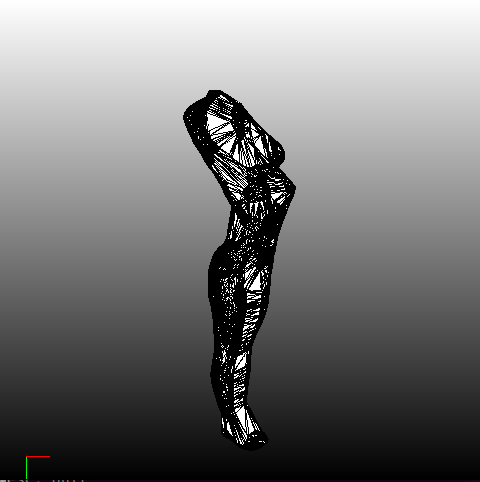
\includegraphics[width=.8\textwidth]{FIGS/alpha/alpha_woman_5k}
        \caption{5 000}
    \end{subfigure}
    \begin{subfigure}{.22\textwidth}
        \centering
        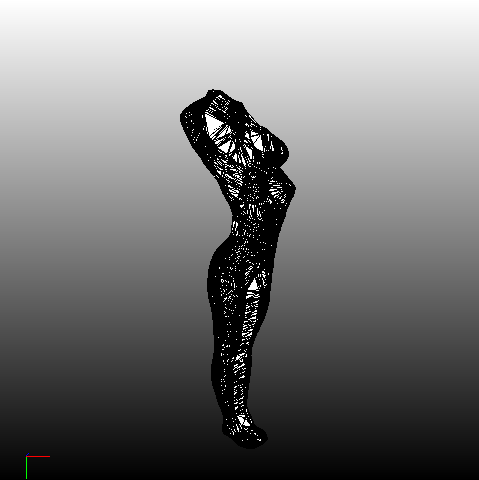
\includegraphics[width=.8\textwidth]{FIGS/alpha/alpha_woman_2k}
        \caption{2 000}
    \end{subfigure}
    \caption{Alpha shape: woman}
    \label{fig:alpha_woman}
\end{figure}


It is clearly seen from given figures, that alpha shaping works good – resulting figures looks better and better with alpha parameter decreasing. Bunt in some moment figures begin to fall apart into separate fragments (“crumble”). Such behavior quite expected cause smaller alpha means less tetrahedrons/triangles in result and in some moment Delaunay triangulation capacity for given region of the figure would be drained completely as it seen from given bunny model.

\section{Crust algorithm}
The idea of Crust for surface reconstruction is proposed by Nina Amenta et al. \cite{abk-anvra-98} in 1998.
Briefly, the crust of a set of points is a set of edges (in 2d) or triangles (in 3d) whose circumcircles is empty of
(1) input points and (2) the medial axis.  A complete crust algorithm is shown in Fig.~\ref{alg:crust-alg}.

Given algorith was implemented in steps.

\begin{enumerate}
    \item At first, the convex hull of point has been evaluated. The result has been used to estimate the \textbf{average of the outer normals of the adjacent triangles} for those points that lie on the convex hull.
    \item 2. Then, the poles has been found by dummy brute-force technique: loop through all points and:
    \begin{enumerate}
        \item If the given point doesn't lie on the convex hull find it's \textbf{positive pole} – farthest Voronoi vertex(the circumsphere of Delaunay tetrahedron was assumed to be the Voronoi vertex) for the given point (to find the farthest Voronoi vertex all them were looped). Vector that goes from point to it's positive pole has been memorized as \textbf{n vector}.
        \item If the given point lie on the convex hull then estimated on the first step \textbf{average of the outer normals of the adjacent triangles} has been memorized as \textbf{n vector}
        \item The \textbf{negative pole} – farthest Voronoi vertex that is located in opposite to \textbf{n vector} direction. To deal with this condition, all Voronoi vertex were looped and in maximization procedure only those vertex has been counted that is seen from the given point on small enough angle in respect to \textbf{n vector}: filtration has been done by cosine of the angle between \textbf{n vector}  and vector that goes from the given point to Voronoi vertex (cosine has been estimated through the scalar product), only Voronoi vertex with cosine in range of [-0.1 0.1]  (or smaller) has been considered in maxmimization procedure.
    \end{enumerate}
    \item  Finally, Delaunay triangulation has be provided for union of points and found poles (both negative and positive). The output (result) has been filtered: only triangles without poles in their content has been counted and used to build figure.
\end{enumerate}

Results are shown on fig.~\ref{fig:crust}
\begin{figure}[h]
    \begin{subfigure}{.5\textwidth}
        \centering
        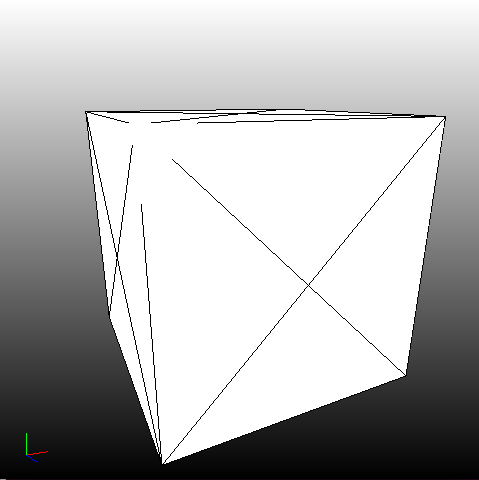
\includegraphics[width=.8\textwidth]{FIGS/crust/crust_cube}
        \caption{Cube: Crust}
    \end{subfigure}
    \begin{subfigure}{.5\textwidth}
        \centering
        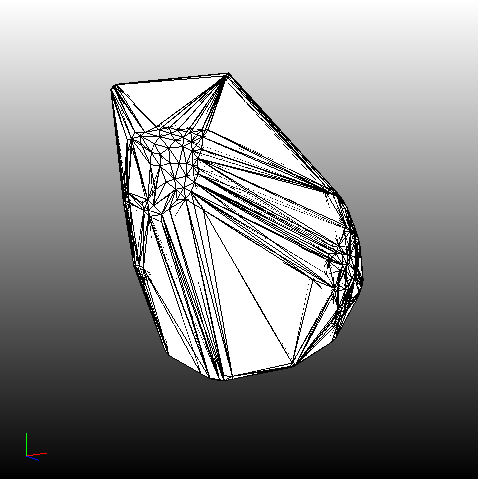
\includegraphics[width=.8\textwidth]{FIGS/crust/crust_bunny}
        \caption{Bunny: Crust}
    \end{subfigure}
    \caption{Crust}
    \label{fig:crust}
\end{figure}


\begin{figure}[h]
    \centering
    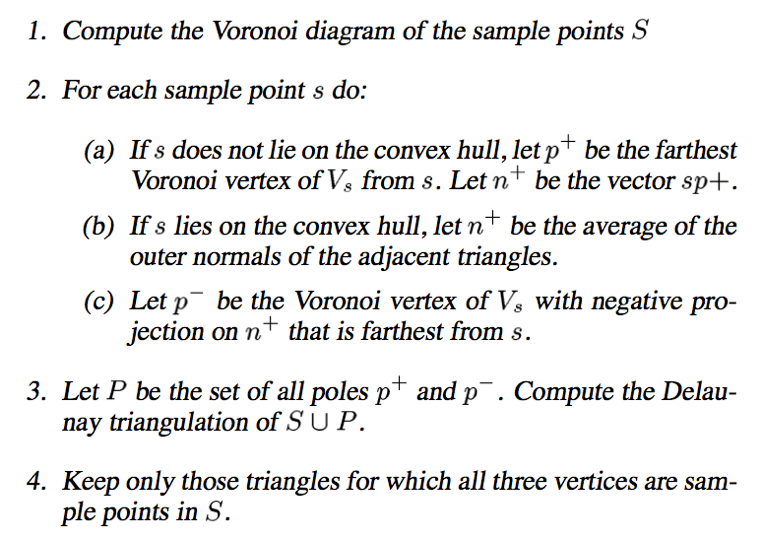
\includegraphics[width=.5\textwidth]{FIGS/crust-alg}
    \caption{3D crust algorithm}
    \label{alg:crust-alg}
\end{figure}

\bibliographystyle{plain}
\bibliography{report}

\end{document}


